\chapter{Desenvolvimento}
\label{chap:Desenvolvimento}

% Descrição de todo o trabalho realizado e dos procedimentos experimentais.

% Resumo opcional. Comentar se não usar.
% \resumodocapitulo{Resumo opcional.}


\section{Biblioteca} \label{sec:lib}
\par O servidor da partida apresenta, como já mencionado na Subseção \ref{subsec:server}, um protocolo de comunicação e sintaxe de mensagens específicos. Uma biblioteca de interfaceamento foi desenvolvida com o objetivo de abstrair os detalhes de comunicação e de construção de mensagens e facilitar, assim, o desenvolvimento dos programas jogadores. Esta abordagem já é comum na categoria e existem soluções de código aberto como a \textit{librcsc}, utilizada por várias equipes, usualmente atreladas ao agente base \textit{agent2d}, desenvolvidas pela equipe \textit{HELIOS}, como visto na Subseção \ref{subsec:abordagens}.
\par A biblioteca própria foi desenvolvida em linguagem Go como forma de modernização e diversificação da base de código utilizada pelas equipes. A biblioteca cobre uma parte considerável das possibilidades previstas no protocolo de comunicação e foi programada de modo a ser facilmente expansível de acordo com o lançamento de atualizações do servidor.

\subsection{Arquitetura do código}
A biblioteca possui três pacotes internos: \textit{playerclient}, \textit{trainerclient} e \textit{rcsscommon}. Os dois primeiros dizem respeito aos dois tipos de programas que podem se conectar ao servidor da partida: jogadores e treinadores. O terceiro engloba todas as funcionalidades utilizadas por ambos clientes, além de informações gerais sobre parâmetros da partida, como coordenadas de bandeiras do campo e modos de jogo.

Os dois clientes desenvolvidos possuem as funcionalidades necessárias para se conectar ao servidor, ouvir mensagens via protocolo UDP, decodificá-las e então executar uma ação em forma de mensagem codificada e enviada ao servidor.

\subsection{Decodificação e Codificação de Mensagens}
\label{sec:messages}
% lexer -> analisador léxico
% parser -> analisador sintático
A decodificação de mensagens, por sua vez, foi feita em duas camadas: um analisador léxico e um analisador sintático. O analisador léxico passa pelas mensagens em formato \textit{string} e identifica os símbolos que ela contém. O analisador sintático extrai desses símbolos as informações e as organiza em estruturas de dados para que possam ser utilizadas fora da biblioteca. As informações recebidas e decodificadas são, em sua maioria, dados dos sensores do jogador.
\begin{center}

\begin{tabular}{c}
\begin{lstlisting}
(see 37 ((f c b) 16.6 -1 -0 -0.8))
\end{lstlisting}
\end{tabular}

Exemplo de mensagem codificada.

\hfill


\begin{tabular}{c}
\begin{lstlisting}
SightSymbols{
	Time: 37,
	ObjMap: map[string][]string{
		"f c b":    {"16.6", "-1", "-0", "-0.8"},
	},
}
\end{lstlisting}
\end{tabular}

Mensagem após passar pelo analisador léxico.

\hfill


\begin{tabular}{c}
\begin{lstlisting}
SightData{
	Time: 37,
	Ball: nil,
	Lines: LineArray{},
	Flags: FlagArray{
		{
			ID:        rcsscommon.FlagCenterBot,
			Distance:  16.6,
			Direction: -1,
		},
	},
}
\end{lstlisting}
\end{tabular}

Mensagem após passar pelo analisador sintático.

\end{center}

\section{Definição dos Estados}
\par As informações de estado são fornecidas pelos sensores do jogador. Há três sensores presentes que entregam informações em forma de mensagens para o agente: sensor auditivo, sensor visual e sensor corporal.
\par Além de ser necessário decodificar as mensagens recebidas, como demonstrado na Subseção \ref{sec:messages}, é necessário processar os dados dos sensores para extrair mais características do estado atual do agente. 

\subsection{Sensores}
\par Os sensores são responsáveis por todas as informações que o jogador tem do ambiente. Eles são modelados de forma a emular características de sensores reais, portanto um sensor pode ``perder'' informações caso o objeto da variável medida esteja longe, como será evidenciado no modelo do sensor visual.

\subsubsection{Sensor Auditivo}

As mensagens do sensor auditivo são do seguinte formato:

\textit{(hear Tempo Remetente "mensagem")}

Onde \textit{Tempo} é o número do ciclo em que a mensagem foi ouvida e \textit{Remetente} é descrição de quem enviou a mensagem. O \textit{Remetente} pode ser o árbitro, outros jogadores, um dos treinadores ou o próprio jogador.

No escopo deste trabalho, apenas as mensagens do árbitro serão consideradas, não sendo implementada nenhuma forma de comunicação direta entre os agentes.

\subsubsection{Sensor Visual}
\label{sec:visual}
As mensagens do sensor visual contém as posições relativas referentes a cada objeto dentro do campo de visão do jogador. Esses objetos podem ser outros jogadores, marcadores como bandeiras e linhas (Figura \ref{fig:flags}) e a bola. O formato genérico é este:

\textit{(see (Objeto1)(Objeto2)(Objeto3)...(ObjetoN))}

Onde cada objeto tem o seguinte formato:

\textit{((NomeDoObjeto) Distância Direção VariaçãoDeDistância VariaçãoDeDireção DireçãoDoCorpo DireçãoDaCabeça)}

Sendo a distância e a direção dados em coordenadas polares, assim como suas variações. As informações de direção do corpo e da cabeça só aparecem quando o objeto em questão é um outro jogador.

O campo é marcado com vários indicadores com posição fixa conhecida para que o agente possa estimar sua posição absoluta, como vista na Figura \ref{fig:flags}.

\begin{figure}[H]
	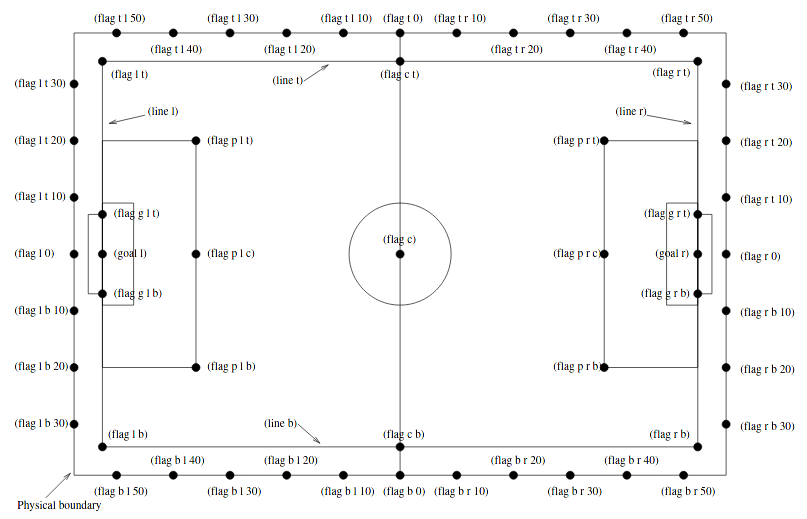
\includegraphics[width=0.9\linewidth]{figs/flags.png}
	\centering
	\caption{Indicadores espalhados pelo campo  \cite{rcssmanual2003}.}
	\label{fig:flags}
\end{figure}

A riqueza de detalhes a respeito das informações obtidas depende da distância entre o objeto e o jogador. Por exemplo, caso um outro jogador esteja sendo visto a uma distância muito grande, pode ser impossível determinar o número de sua camisa ou até mesmo a qual time ele pertence. Em contrapartida, para jogadores próximos, é fornecido até mesmo a direção para a qual ele está olhando.

\subsubsection{Sensor Corporal}

O sensor corporal contém informações sobre o estado físico do jogador. Entre elas sua energia, que é consumida a cada ação tomada como chute ou arrancada (Subseção \ref{sec:actions}), sua própria velocidade e direção de movimento, a direção de sua cabeça e a quantidade de cartões de advertência recebidos.

\subsection{Estimação e Tratamento de Estados}

\par Os sensores do jogador fornecem somente informações em coordenadas polares relativas ao próprio jogador. Desta forma, ele possui informações de distância e direção para a bola, demais jogadores, bandeiras do campo e linhas do campo.

\par Com esses dados é possível estimar as coordenadas cartesianas absolutas no campo de todas as entidades de interesse. As bandeiras do campo são fixas e possuem coordenadas conhecidas, detalhado na subseção \ref{sec:visual}. Logo, a transformação da informação polar e relativa para uma cartesiana e absoluta da posição do próprio jogador é direta utilizando trigonometria básica. 

\par A partir da informação de posição absoluta do próprio jogador é possível calcular as posições absolutas para o resto das entidades.

% \par É possível também extrair estados úteis a partir das informações dos sensores, como por exemplo um estado que representa há quantos ciclos de simulação o jogador não vê a bola. Este estado pode ser determinante para que o jogador escolha, por exemplo, tomar a decisão de buscar a bola para atualizar a informação que possui sobre ela.


\section{Definição de Ações}

\par Os jogadores possuem diversas ações possíveis mapeadas pelo servidor da partida. As ações recebem parâmetros em sua maioria contínuos. Dessa forma a escolha de quais ações devem ser executadas se dá em um domínio discreto, porém cada ação exige uma escolha de parâmetros em um domínio contínuo.

\subsection{Arrancar}
\label{sec:dash}

O comando de arrancar faz com que haja uma aceleração do jogador na direção da arrancada. O parâmetro ``potência'' determina o valor da aceleração e o parâmetro ``direção'' é relativo à direção do corpo do jogador. É importante salientar que o comando de arranque é o jeito padrão de movimentar um jogador.

Cada jogador possui uma certa quantidade de energia e o arranque tem um custo sobre ela. Ao começo de cada partida, a energia do jogador é colocada no máximo. Se o jogador acelera para frente, a energia é reduzida em $1\times$ a potência. Se o jogador acelera para trás, o custo é maior e a energia é reduzida em $2\times$ a potência.

Se a energia disponível é menor que a necessária para a realização com comando, o valor de ``potência'' é reduzido para que a quantidade necessária de energia seja a disponível.

\subsection{Chutar}

O comando de chute recebe dois parâmetros: a força e a direção do chute. Para realizar o comando, a bola precisa ser ``chutável'', ou seja, estar a uma certa distância do jogador.

Caso a bola não esteja diretamente à frente do jogador, a força efetiva será reduzida por um fator dependente da posição relativa da bola.

\subsection{Virar}

O comando virar recebe como parâmetro o momento angular a ser aplicado pelo jogador sobre si mesmo. Se o jogador não estiver em movimento, o seu ângulo é apenas incrementado com o momento.

Porém, caso o jogador esteja em movimento, o resultado do comando é influenciado pelo momento de inércia do jogador (definido aleatoriamente pelo servidor no início da partida) e sua velocidade linear.

\subsection{Virar pescoço}

O jogador pode virar seu pescoço de maneira semi-independente de seu corpo. O ângulo do pescoço é relativo ao ângulo do corpo, então caso um comando virar seja executado, o ângulo absoluto do pescoço também mudará. Os ângulos máximo e mínimo em relação ao corpo são definidos na configuração do servidor, sendo o padrão +90 e -90 graus, respectivamente.

\subsection{Mover-se}
\label{sec:move}

O comando ``mover-se'' é utilizado para mover diretamente jogadores para coordenadas. Não pode ser utilizado no decorrer de uma partida, exceto quando o goleiro tem a posse da bola. O comando fica disponível no início dos tempos da partida para posicionamento dos jogadores.

Para movimentar os jogadores durante a partida, o arranque (Subseção \ref{sec:dash}) deve ser utilizado.

% TODO: remover essa seção? nem falamos nada direito do goleiro o artigo inteiro...
\subsection{Agarrar}

O único jogador com permissão para agarrar ou pegar a bola é o goleiro. O goleiro pode pegar a bola em qualquer direção, desde que ela esteja dentro da área agarrável (Figura \ref{fig:catch}), definida como um retângulo com comprimento 2.0 e largura 1.0 na direção em que se deseja tentar agarrar.

Se o comando de agarrar falhar o goleiro fica incapacitado de agarrar a bola durante um número pré-determinados de ciclos do jogo. Se o comando tiver sucesso o goleiro pode usar o comando "mover-se" (Seção \ref{sec:move}) para se mover segurando a bola até um limite máximo de vezes estabelecido nas configurações do servidor.

\begin{figure}[H]
	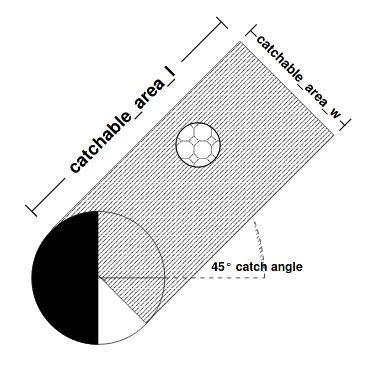
\includegraphics[width=0.5\linewidth]{figs/catch.png}
	\centering
	\caption{Visualização da área agarrável pelo goleiro \cite{rcssmanual2003}.}
	\label{fig:catch}
\end{figure}

\subsection{Falar}

Usado para transmitir mensagens aos outros jogadores. As mensagens devem ter comprimento menor que um valor pré-determinado pelo servidor. Os jogadores que estiverem a uma distância audível da mensagem receberão a mensagem do servidor imediatamente.

Não será implementada nenhuma comunicação entre os jogadores neste trabalho.


\section{Ambiente de Treinamento}

O ambiente de treinamento consiste em uma base de código que importa a biblioteca detalhada na Seção \ref{sec:lib}. Um formato geral foi definido e desenvolvido a fim de tornar os experimentos fáceis de adaptar, bastando mudar alguns trechos do código.

\subsection{Laço de Treinamento}

De forma geral o laço de treinamento obedece ao pseudo-código apresentado.

\begin{tabular}{c}
	\begin{lstlisting}
		definir parametros
		inicializar pesos de treinamento
		enquanto o estado nao e terminal:
			conectar jogador
			para cada ciclo da partida:
				escolher acao de acordo com a politica e o estado
				observar novo estado e recompensa
				treinar pesos
				estado <- novo estado
	\end{lstlisting}
\end{tabular}

O laço interno é onde efetivamente os algoritmos de treinamento são implementados, portanto este trecho é alterado a depender da técnica de aprendizagem por reforço utilizada.


\section{Experimentos}

O objetivo inicial para teste do sistema como um todo foi o de realizar o treinamento de um agente único capaz de executar gols estando sozinho em campo.

Para isso foram realizadas três abordagens diferentes.

\begin{itemize}
	\item Sarsa com método aproximado e comportamentos pré-programados
	\item Double Q-Learning tabular e comportamentos pré-programados
	\item Double Q-Learning tabular e ações puras
\end{itemize}

\subsection{Sarsa Aproximado e Comportamentos Pré-Programados}

Inicialmente, desejou-se realizar um treinamento utilizando um método aproximado, devido ao grande número de estados contínuos possíveis para o agente. Portanto, foi usada uma rede neural multicamada com estrutura detalhada na Tabela \ref{table:ann}.

\begin{table}[h]
	\centering
	\begin{tabular}{||c c||} 
		\hline
		camada & nº neurônios  \\ [0.5ex] 
		\hline\hline
		1 & 5  \\ 
		\hline
		2 &  256 \\
		\hline
		3 & 256 \\
		\hline
		4 & 128  \\
		\hline
		5 & 64 \\ 
		\hline
		6 & 8 \\ [1ex] 
		\hline
	\end{tabular}
	\caption{Estrutura da rede neural utilizada no experimento}
	\label{table:ann}
\end{table}

A utilização de comportamentos permite que sejam inseridos conhecimentos prévios a respeito do que é esperado de um agente jogador de futebol, ou seja, é possível simplificar o aprendizado substituindo as ações puras como chutar ou correr por ações abstratas como perseguir a bola e chutar para o gol.

\subsubsection{Codificação dos Estados}
\label{subsubsec:state-approx}


\begin{itemize}
	\item \textbf{Coordenada X do Jogador}: dentro do intervalo $[-1, 1]$ e normalizada em relação ao comprimento do campo.
	\item \textbf{Coordenada Y do Jogador}: dentro do intervalo $[-1, 1]$ e normalizada em relação à largura do campo.
	\item \textbf{Orientação do Jogador}: dentro do intervalo $[-1, 1]$ e proporcional ao ângulo do corpo do jogador em relação ao eixo X entre $-180^{\circ}$ e $180^{\circ}$.
	\item \textbf{Distância até a bola}: normalizada em relação à distância máxima visível.
	\item \textbf{Direção da bola}: dentro do intervalo $[-1, 1]$ e proporcional ao ângulo do corpo do jogador em relação ao vetor que o liga à bola entre $-180^{\circ}$ e $180^{\circ}$. 
	
\end{itemize}

\subsubsection{Codificação dos Comportamentos}
\label{subsubsec:behaviors-mapping}
Os comportamentos pré-programados foram desenvolvidos de forma a cobrir ações que permitissem a realização de gols, que é o objetivo do treinamento.

\begin{itemize}
	
	\item \textbf{Comportamento nulo}: O agente apenas espera até o próximo ciclo.
	
	\item \textbf{Localizar bola}: Caso o agente não veja a bola, ele gira no seu próprio eixo na direção em que a bola foi vista pela última vez. Se a bola não foi vista por mais de 30 ciclos, o agente gira em seu eixo $45^{\circ}$, a fim de achar a bola mais rápido. 
	
	\item \textbf{Se aproximar da bola}: Caso o agente veja a bola, ele se move em direção a ela com velocidade constante
	
	\item \textbf{Se afastar da bola}: Caso o agente veja a bola, ele se move em direção oposta a ela com velocidade constante
	
	\item \textbf{Carregar bola para o gol direito}: Caso a distância até a bola seja menor ou igual a 0.7 metros, o agente chuta levemente a bola e anda de forma a conduzi-la ao gol direito.
	
	\item \textbf{Chutar bola para gol direito}: Caso a distância até a bola seja menor ou igual a 0.7 metros, o agente chuta a bola na direção do gol direito.
	
	\item \textbf{Carregar bola para o gol esquerdo}: Caso a distância até a bola seja menor ou igual a 0.7 metros, o agente chuta levemente a bola e anda de forma a conduzi-la ao gol esquerdo.
	
	\item \textbf{Chutar bola para gol esquerdo}: Caso a distância até a bola seja menor ou igual a 0.7 metros, o agente chuta a bola na direção do gol esquerdo.
	
\end{itemize}

\subsubsection{Parâmetros}
\label{subsubsec:sarsa-params}

% TODO: mudar os parâmetros dependendo do Sarsa utilizado
\begin{itemize}
	\item \textbf{Fator de desconto ($\gamma$)}: Apesar do ambiente ser episódico, foi utilizado um fator de desconto de 0.99 devido ao fato de que a condição de término do episódio (fim de jogo) não ser observável através da discretização do estado utilizada.  
	
	\item \textbf{Fator de aprendizagem ($\alpha$)}: O fator de aprendizagem foi definido inicialmente como 0.1 e foi reduzido exponencialmente multiplicando-o por $0.99999$ ao final de cada partida. 
	
	\item \textbf{Fator de exploração ($\epsilon$)}: Para incentivar a exploração das possibilidades, o fator de exploração foi definido inicialmente como 0.9 e reduzido exponencialmente multiplicando-o por $0.99996$ ao final de cada partida. A cada ação tomada, o agente tem probabilidade $\epsilon$ de escolher uma ação aleatória. Além disso, para favorecer a exploração, no início de cada partida era também sorteada uma posição inicial para o agente em seu lado do campo.
\end{itemize}

\subsubsection{Recompensa}
\label{subsubsec:reward}

A recompensa foi definida em 3 partes a fim de guiar o agente na direção do aprendizado desejado. Todas as medições de recompensa foram feitas utilizando dados da simulação e não da percepção do agente.

\begin{itemize}
	\item \textbf{Proximidade da bola $R_1$}: Para que o agente tenha tendência a se aproximar da bola, foi definida uma recompensa negativa proporcional à distância $d$ do agente em relação à bola, ou seja: $R_1 = -d*0.001/6000$.
	
	\item \textbf{Velocidade da bola $R_2$}: Para que o agente adquira o comportamento de chutar a bola em direção ao gol adversário, foi definida uma recompensa positiva proporcional à velocidade instantânea da bola em X ($v_x$), ou seja: $R_2 = v_x/6000$.
	
	\item \textbf{Gol $R_3$}: Por fim, para incentivar que o agente fizesse gols, foi definida uma recompensa esparsa de valor 1 para cada gol realizado e -1 para gols contra, ou seja:
	
	$
	R_3 =
	\left\{
	\begin{array}{ll}
		\ \ 1  & \mbox{se foi feito um gol no ciclo} \\
		-1  & \mbox{se foi feito um gol contra no ciclo} \\
		\ \ 0  & \mbox{caso não houver gol no ciclo} \\
	\end{array}
	\right.
	$
\end{itemize}

Deste modo, a cada instante de tempo foi atribuída uma recompensa $R = R_1 + R_2 + R_3$.

\subsection{Double Q-Learning Tabular e Comportamentos Pré-Programados}

Além da solução através de um aproximador de funções, foi testada uma solução utilizando o método tabular com os mesmos comportamentos e uma discretização dos estados descrita abaixo.

A codificação dos comportamentos, parâmetros $\alpha$, $\epsilon$ e $\gamma$ e a recompensa foram mantidos como descrito nas subseções \ref{subsubsec:behaviors-mapping}, \ref{subsubsec:sarsa-params} e \ref{subsubsec:reward} respectivamente.

\subsubsection{Codificação dos Estados}
\label{subsubsec:state-encoding}

O estado percebido pelo agente é dado pela combinação dos seguintes fatores:

\begin{itemize}
	\item \textbf{Distância até a bola}. A distância $D$ até a bola foi discretizada de acordo com a seguinte função:
	\begin{equation}
		\label{eq:balldist}
		\left\{
		\begin{array}{ll}
			0  & \mbox{se } D < 0.7 \\
			\lfloor\log_2 (\frac{D}{0.7})\rfloor & \mbox{se } 0.7 \leq D \mbox{ e } D < 0.7 \times 2^6 \\
			6  & \mbox{se } D \geq 0.7 \times 2^6 \\
			
		\end{array}
		\right.
	\end{equation}
	
	Ou seja, a distância percebida até a bola varia entre 0 e 6 com resolução cada vez menor à medida que o agente se afasta da bola. O fator 0.7 foi inserido na função devido ao fato de que esta é a distância mínima que permite que o agente chute a bola.
	
	Caso o jogador possa enxergar a bola, a distância D é recebida diretamente do sensor. Caso contrário, a distância D é estimada com base na última posição percebida da bola.
	
	\item \textbf{Direção da bola}: A direção da bola foi dividida em 24 fatias de $15^{\circ}$ cada. O ângulo de visão do jogador é de $\pm30^{\circ}$. Caso a bola não esteja visível, a direção da bola é estimada com base na última posição percebida.
	
	\item \textbf{Posição do jogador em X}: A posição estimada do jogador em X foi discretizada em 10 janelas de tamanho $11.5$.
	
	\item \textbf{Posição do jogador em Y}: A posição estimada do jogador em Y foi discretizada em 7 janelas de tamanho aproximado $11.14$.
	
	\item \textbf{Direção do jogador}: A direção estimada do jogador em relação ao eixo horizontal foi discretizada em 24 fatias de $15^{\circ}$ cada.
	
\end{itemize}

Com isso, temos que o número total de estados possíveis é dado pelo produtório da quantidade de possibilidades em cada um dos itens acima totalizando 282240 estados.

\subsection{Double Q-Learning Tabular e Ações Puras}
% Inicialmente, deseja-se realizar o treinamento de um agente único que, com as informações de seus sensores, consiga com sucesso levar a bola ao gol. Essa proposta tem como objetivo fundamentar os conhecimentos e validar a base de código para a realização de um treinamento de um time de múltiplos agentes em um estágio posterior.

% O desenvolvimento de um agente único, inicialmente, permite adquirir o entendimento necessário para a definição do vetor de estados e ajuste das técnicas de treinamento. Além disso, busca-se uma maior agilidade na substituição e teste na estrutura do vetor de estados e no algoritmo de treinamento, uma vez que o custo computacional deste cenário é consideravelmente menor que o custo do treinamento de um time completo.

% Esse objetivo se provou mais difícil do que o esperado para a abordagem \textit{end-to-end} desejada.

% TODO: detalhar mais

Após o resultado positivo obtido utilizando comportamentos pré-programados, foi testada uma abordagem \textit{end-to-end} utilizando a discretização de estados descrita na subseção \ref{subsubsec:state-encoding} e a recompensa descrita na subseção \ref{subsubsec:reward}.

% Foi utilizado o algoritmo Double Q-Learning tabular, possível através da discretização de diversas métricas obtidas através dos sensores do agente.

\subsubsection{Codificação das Ações}

Para simplificar o vasto espaço de ações disponíveis, foi selecionado um conjunto discreto de 13 ações:

\begin{itemize}
	\item \textbf{Ação nula}: O agente apenas espera até o próximo ciclo.
	
	\item \textbf{Virar-se}: O agente tem a opção de virar-se $7^{\circ}$, $15^{\circ}$ ou $31^{\circ}$ para ambas as direções, totalizando 6 ações de rotação possíveis. 
	
	\item \textbf{Correr}: É possível correr em frente ($0^{\circ}$) ou a $30^{\circ}$ em ambas as direções, sempre com potência 50, totalizando 3 ações de corrida possíveis.
	
	\item \textbf{Chutar}: Caso a distância até a bola seja menor ou igual a 0.7 metros, o jogador tem a opção de chutá-la em frente ou em um ângulo de $45^{\circ}$ em ambas as direções, totalizando 3 ações de chute possíveis. Caso a bola não esteja próxima o suficiente, nada acontece.
\end{itemize}

\subsubsection{Parâmetros}
\label{subsubsec:tabular-params}

\begin{itemize}
	\item \textbf{Fator de desconto ($\gamma$)}: Foi mantido tal como descrito na subseção \ref{subsubsec:sarsa-params}.
	
	\item \textbf{Fator de aprendizagem ($\alpha$)}: O fator de aprendizagem foi definido como $\frac{6000}{6000+N}$ sendo $N$ o número de partidas experienciadas pelo jogador. 
	
	\item \textbf{Fator de exploração ($\epsilon$)}: O fator de aprendizagem foi definido como $\frac{8000}{8000+N}$ sendo $N$ o número de partidas experienciadas pelo jogador. 
\end{itemize}